\documentclass[cjk,dvipdfmx,10pt,compress,fragile%
hyperref={bookmarks=true,bookmarksnumbered=true,bookmarksopen=false,%
colorlinks=false,%
pdftitle={第 134 回 関西 Debian 勉強会},%
pdfauthor={小林},%
%pdfinstitute={関西 Debian 勉強会},%
pdfsubject={資料},%
}]{beamer}

\title{Rustで書いたツールのdebianパッケージングに\\挑戦してみた話(仮)}
\author[Katsuki Kobayashi]{{\large\bf Katsuki Kobayashi}}
\institute[Debian JP]{{\normalsize\tt 関西 Debian 勉強会}}
\date{{\small 2019年 3月 24日 (日)}}

\usepackage{graphicx}
\usepackage{moreverb}
\usepackage{ulem}
\usepackage[varg]{txfonts}
\usepackage{tabularx}
\usepackage{fancybox}
\usepackage{fancyvrb}
\usepackage{float}
\usepackage{multicol}
\usepackage{minijs}
\usepackage{amsmath}
\usepackage{amssymb}
\usepackage{newtxtext}
\usepackage{listings, listings-rust}
\usepackage{xcolor}
\usepackage{hyperref}
\AtBeginDvi{\special{pdf:tounicode EUC-UCS2}}
\usetheme{KansaiDebian}
\def\museincludegraphics{%
  \begingroup
  \catcode`\|=0
  \catcode`\\=12
  \catcode`\#=12
  \includegraphics[width=0.9\textwidth]}
%\renewcommand{\familydefault}{\sfdefault}
%\renewcommand{\kanjifamilydefault}{\sfdefault}
%
\newenvironment{commandline}%
{\VerbatimEnvironment
  \begin{Sbox}\begin{minipage}{0.9\hsize}\begin{fontsize}{8}{8} \color{white} \begin{BVerbatim}}%
{\end{BVerbatim}\end{fontsize}\end{minipage}\end{Sbox}
  \setlength{\fboxsep}{8pt}
% start on a new paragraph

\vspace{6pt}% skip before
\fcolorbox{white}{black}{\TheSbox}

\vspace{3pt}% skip after
}
%end of commandline

\begin{document}

\begin{frame}[fragile]
\titlepage
\end{frame}

\begin{frame}[t,fragile]{自己紹介}
 \begin{itemize}
  \item Katsuki Kobayashi
	\begin{itemize}
	 \item 組み込みエンジニア
	 \item 使用言語: C, アセンブラ(ARM)
	 \item \sout{永遠}に勉強中: Python, Kotlin, アセンブラ(RISC-V), Rust
	       \onslide<2>{\item 最近会社でC++を勉強させられている。タスケテ。}
	\end{itemize}
  \item Debianとのつきあい
	\begin{itemize}
	 \item 大学時代に素敵な先輩がた(うち現在DD2名,DM1名)によって布教
	 \item 個人的にはパッケージの構成の統一感が一番好き
	 \onslide<2>{\item \sout{あんまり貢献していない}}
	\end{itemize}
  \item Rust
	\begin{itemize}
	 \item 新しい言語が勉強したい
	 \item でもPythonやRubyはネイティブなバイナリにならなくてツラい
	 \onslide<2>{\item Goが流行ってるらしい}
	 \item じゃあMozilla好きだしRustにしよう \onslide<2>{←?}
	\end{itemize}
 \end{itemize}
\end{frame}

\begin{frame}[t,fragile]{本日の流れ}
\begin{itemize}
 \item Rustをさわってみる
       \begin{itemize}
	\item rustupでツールチェーンをインストール
	\item Cargoでビルドしてみる
       \end{itemize}
 \item Rustの特徴のご紹介
       \begin{itemize}
	\item 注意: 発表者も素人なので難しい質問は回答できません
	\item \url{https://doc.rust-lang.org/stable/book/} を読んでください!!
       \end{itemize}
 \item Debianパッケージングを試してみた話
\end{itemize}
\end{frame}

\begin{frame}[t,fragile]{Rustとは?}
 \begin{itemize}
  \item Mozillaが開発したシステムプログラミング言語
	\begin{itemize}
	 \item Servo(絶賛開発中)というブラウザエンジンのために開発
	 \item 安全性・並行性について考えられて設計されている
	 \item 静的型付け言語
	 \item 学習曲線がツライとうわさ
	\end{itemize}
  \item カニ?
	\begin{itemize}
	 \item Rustプログラマーの事をRustacean(ラストシアン)と呼ぶ
	 \item ``Crustacean(甲殻類)`` から来ているらしい
	       \begin{itemize}
		\item オライリー本の表紙はオオヒロバオウギガニ
		\item 非公式なマスコットもカニ \href{http://rustacean.net/}{(Ferrisっていう模様)}
	       \end{itemize}
	\end{itemize}
  \item Rustのファイルの拡張子は .rs
	\begin{itemize}
	 \item Rustで書かれたプロジェクトの公式サイトが \verb|http://xxx.rs| であることが多い
	 \item 国別コードトップドメイン .rs : セルビア
	\end{itemize}
 \end{itemize}
\end{frame}

\begin{frame}[t,fragile]{インストール}
 \begin{itemize}
  \item \texttt{rustup}を入れるのが一応公式
	\begin{itemize}
	 \item \verb@curl https://sh.rustup.rs -sSf | sh@
	 \item あなたのhome dirに色々と入ります \verb@~/.cargo@
	\end{itemize}
  \item \texttt{rustup}のサブコマンドたち
	\begin{description}
	 \item[default] デフォルトのツールチェーンを切り替えます。
		    \begin{itemize}
		     \item ツールチェーン: stableかnightlyか特定のバージョンを指定できる
		    \end{itemize}
	 \item[update] 更新をかけます。
		    nightlyを使う場合はちょくちょく使う
		    \begin{itemize}
		     \item そしてたまに壊れる
		     \item 壊れるといっても、コンパイラがおかしくなった事はないです
		     \item 10年前くらいのsidの気分を味わえます
		    \end{itemize}
	 \item[completions] シェルの補完用のコードを吐く (bash, zsh, fish, \textbf{PowerShell}, etc..)
	\end{description}
 \end{itemize}
\end{frame}

\begin{frame}[t,fragile]{Debianパッケージでのインストール}
 \begin{itemize}
  \item もちろんDebianのパッケージもある
	\begin{itemize}
	 \item ビルドツールであるcargoのパッケージを入れるのがよろしいかと
	 \item 一緒にコンパイラ(rustc)も入ります
	\end{itemize}
 \end{itemize}
 \begin{commandline}
% apt show cargo
Package: cargo
Version: 0.33.0-1
Priority: optional
Section: rust
Maintainer: Rust Maintainers <pkg-rust-maintainers@alioth-lists.debian.net>
Installed-Size: 9,453 kB
Depends: libc6 (>= 2.18), libcurl3-gnutls (>= 7.28.0), libgcc1 (>= 1:4.2), \
libgit2-27 (>= 0.26.0), libssh2-1 (>= 1.2.5), libssl1.1 (>= 1.1.0), \
zlib1g (>= 1:1.1.4), rustc (>= 1.24), binutils, gcc | clang | c-compiler
Suggests: cargo-doc, python3
Homepage: https://crates.io/
Download-Size: 2,483 kB
APT-Manual-Installed: yes
APT-Sources: http://ftp.jp.debian.org/debian sid/main amd64 Packages
 \end{commandline}
\end{frame}

\begin{frame}[t,fragile]{Hello World (1/4)}
 \begin{itemize}
  \item Rustのプロジェクトは、 \verb|cargo new| で作ります
	\begin{itemize}
	 \item \verb|--bin| (現default) か \verb|--lib| (旧default) でパッケージの種類も指定できます
	\end{itemize}
 \end{itemize}
\begin{commandline}
% cargo new hello
     Created binary (application) `hello` package
\end{commandline}
\begin{itemize}
 \item 実行すると、Cargo.tomlとsrc/main.rsができる
\end{itemize}
\begin{commandline}
% tree
.
├── Cargo.toml
└── src
    └── main.rs

1 directory, 2 files
\end{commandline}
\end{frame}

\begin{frame}[t,fragile]{Hello World (2/4)}
 \begin{itemize}
  \item 実はプロジェクトを作った時点でHello Worldの半分が完了している
	\begin{itemize}
	 \item 生成されたsrc/main.rsの中身↓
	\end{itemize}
 \end{itemize}
\begin{lstlisting}[language=Rust,style=boxed,style=colouredRust,basicstyle=\small\tt,lineskip=-2pt]
fn main() {
    println!("Hello, world!");
}\end{lstlisting}
\begin{itemize}
 \item 実行するには \verb|cargo run|
       \begin{itemize}
	\item 実はデバッグビルドなので、最適化をかけるには\verb|--release|をつける
       \end{itemize}
\end{itemize}
\begin{commandline}
% cargo run
   Compiling hello v0.1.0 (/path/to/hello)
    Finished dev [unoptimized + debuginfo] target(s) in 0.31s
     Running `target/debug/hello`
Hello, world!
\end{commandline}
\end{frame}

\begin{frame}[t,fragile]{Hello World (3/4)}
\begin{itemize}
 \item 少しコードを見てみる
\end{itemize}
\begin{lstlisting}[language=Rust,style=boxed,style=colouredRust,basicstyle=\small\tt,lineskip=-2pt]
fn main() {
    println!("Hello, world!");
}\end{lstlisting}
 \begin{description}
  \item[関数定義] \verb|fn|を使う
  \item[main関数] 戻り値は書かない
  \item[\texttt{println!()}] 実は関数ではなくてマクロ (\verb|!|が付いてるのはマクロ)
 \end{description}
\end{frame}

\begin{frame}[t,fragile]{Hello World (4/4)}
\begin{itemize}
 \item Cargo.toml
\end{itemize}

\begin{commandline}
[package]
name = "hello"
version = "0.1.0"
authors = ["Katsuki Kobayashi <katsuki.kobayashi@gmail.com>"]
edition = "2018"

[dependencies]
\end{commandline}

\begin{itemize}
 \item Cargo.lock (ビルドすると自動生成)
\end{itemize}

\begin{commandline}
# This file is automatically @generated by Cargo.
# It is not intended for manual editing.
[[package]]
name = "hello"
version = "0.1.0"
\end{commandline}
\end{frame}

\begin{frame}[t,fragile]{それじゃあ……}
\begin{itemize}
 \item ちょっと色々とRustの構文とか機能を紹介します
       \begin{itemize}
	\item 解らない or もっと詳しくと思ったらThe bookを読んでもらえればと
	      \begin{itemize}
	       \item 口頭で聞いてもらっても良いですが回答に窮する可能性が高いです \verb|;-)|
	      \end{itemize}
	\item The book: \url{https://doc.rust-lang.org/stable/book/}
	\item 実行環境はwebでやってもらっても良いかもです
	      \begin{itemize}
	       \item \url{https://play.integer32.com/}
	      \end{itemize}
       \end{itemize}
 \item まじめに向き合うには結構大変
       \begin{itemize}
	\item カニ本で引用されてる
	      \href{https://www.quora.com/What-do-C-C++-systems-programmers-think-of-Rust/answer/Mitchell-Nordine}{Quoraの記事}
	\item C++の本を現在進行形で読んでる身にはすごく納得
	      \begin{itemize}
	       \item 大体、C++11ではこう書けるからそれが推奨っていうのがRustの文法
	      \end{itemize}
       \end{itemize}
\end{itemize}
\begin{quote}
I've found that Rust has forced me to learn many of the things that I was slowly learning as "good practise" in C/C++ before I could even compile my code.
\end{quote}
\end{frame}

\begin{frame}[t,fragile]{変数宣言(1/3)}
\begin{lstlisting}[language=Rust,style=boxed,style=colouredRust,basicstyle=\small\tt,lineskip=-2pt]
    let x = 1;
    println!("x = {}", x);
    let x = 1.25;
    println!("x = {}", x);
    // x = 1;   // error: expected floating-point number,
                // found integer
    // x = 1.5; // error: cannot assign twice to
                // immutable variable\end{lstlisting}
\begin{itemize}
 \item 変数の宣言はletで行なう
       \begin{itemize}
	\item 型は(一意に推論できるなら)省略可能
	\item シャドーイング可能
	\item 指定がなければimmutableな変数になる
       \end{itemize}
\end{itemize}
\end{frame}

\begin{frame}[t,fragile]{変数宣言(2/3)}
\vspace*{-2zw}
\begin{lstlisting}[language=Rust,style=boxed,style=colouredRust,basicstyle=\small\tt,lineskip=-2pt]
    let mut y: u32 = 1;
    y -= 1;
    y -= 1;
    println!("y = {}", y);\end{lstlisting}
\begin{itemize}
 \item 変数の宣言はletで行なう
       \begin{itemize}
	\item 型は後置貴方(コロンの後ろにつける)
	\item mutableな変数にしたければ \texttt{mut} キーワードを使う
       \end{itemize}
 \item ちなみに、実行するとデバッグビルドだと途中で止まります
\end{itemize}
\begin{commandline}
% cargo run
Compiling variable v0.1.0 (/path/to/examples/variable)
Finished dev [unoptimized + debuginfo] target(s) in 0.00s
Running `target/debug/variable`
thread 'main' panicked at 'attempt to subtract with overflow', \
variable/src/main.rs:12:5
note: Run with `RUST_BACKTRACE=1` environment variable to \
display a backtrace.
\end{commandline}
\end{frame}

\begin{frame}[t,fragile]{変数宣言(3/3)}
 \begin{itemize}
  \item リリースビルド(\verb|--release|付き)すると最後まで実行する
	\begin{itemize}
	 \item もちろん、結果はおかしなことになる
	\end{itemize}
 \end{itemize}
\begin{commandline}
% cargo run
Compiling variable v0.1.0 (/path/to/examples/variable)
Finished release [optimized] target(s) in 0.30s
Running `target/release/variable`
x = 1
x = 1.25
y = 4294967295
\end{commandline}
\end{frame}

\begin{frame}[t,fragile]{基本的な型}
 \begin{description}
  \item[整数]
	      \textbf{符号無し:} \texttt{u8}, \texttt{u16}, \texttt{u32}, \texttt{u64}, \texttt{usize}\\
	      \textbf{符号付き:} \texttt{i8}, \texttt{i16}, \texttt{i32}, \texttt{i64}, \texttt{isize}
  \item[浮動小数点] \textbf{単精度:} \texttt{f32}、\textbf{倍精度:} \texttt{f64}
  \item[ブール] \texttt{bool}
  \item[文字] \texttt{char}  (Unicodeの1文字)
  \item[文字列] \texttt{String}
	     \begin{itemize}
	      \item ただし、文字列リテラルの \texttt{str} があってとてもややこしい
	     \end{itemize}
  \item[配列] \texttt{[T; N]} (\texttt{T}: 型,  \texttt{N}: 要素数)
  \item[ベクター] \texttt{Vec<T>} (\texttt{T}: 型)
  \item[スライス] \texttt{\&[T]} (\texttt{T}: 型)
 \end{description}
\end{frame}

\begin{frame}[t,fragile]{\texttt{String}と\texttt{str} (1/2)}
\begin{itemize}
 \item C++の\texttt{std::string}と\texttt{char}に似ている
\end{itemize}
\begin{lstlisting}[language=Rust,style=boxed,style=colouredRust,basicstyle=\small\tt,lineskip=-2pt]
    let a = "abcd".to_string(); // String::from("abcd"); も可
    let b = &a[1..];
    let c = "zyxwv";\end{lstlisting}
\begin{center}
 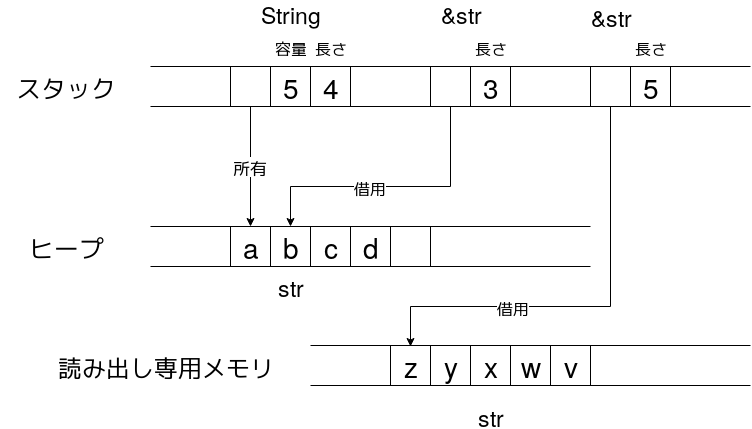
\includegraphics[keepaspectratio,height=4cm]{./img/rustlang-str-string.png}
\end{center}
\end{frame}

\begin{frame}[t,fragile]{\texttt{String}と\texttt{str} (2/2)}
\begin{itemize}
 \item \texttt{String}は可変長
\end{itemize}
\begin{lstlisting}[language=Rust,style=boxed,style=colouredRust,basicstyle=\small\tt,lineskip=-2pt]
    let mut a = "abcd".to_string();
    //  ^^^
    a.push_str("efg");  // OK

    let mut c = "zyxwv";
    // no method named `push_str` found
    // for type `&str` in the current scope
    c.push_str("ut");  // Error!! \end{lstlisting}
\end{frame}

\begin{frame}[t,fragile]{関数}
 \begin{itemize}
  \item \texttt{fn} キーワードと \texttt{->} トークンを使って書く
 \end{itemize}
\begin{lstlisting}[language=Rust,style=boxed,style=colouredRust,basicstyle=\small\tt,lineskip=-2pt]
fn add(a: i32, b: i32) -> i32 {
    return a + b;
}

fn main() {
    println!("{}", add(1, 2));
}\end{lstlisting}

\begin{commandline}
% cargo run
Compiling function v0.1.0 (/path/to/examples/function)
Finished dev [unoptimized + debuginfo] target(s) in 0.20s
Running `target/debug/function`
3
\end{commandline}
\end{frame}

\begin{frame}[t,fragile]{所有権(1/4)}
 \begin{itemize}
  \item 整数型と文字列型の変数を複数の変数に代入してみる
	\begin{itemize}
	 \onslide<2>{\item どうなると思います?}
	\end{itemize}
 \end{itemize}
 \begin{lstlisting}[language=Rust,style=boxed,style=colouredRust,basicstyle=\small\tt,lineskip=-2pt]
    let i0 = 1;
    let i1 = i0;
    let i2 = i0;

    let s0: String = "hoge".to_string();
    let s1 = s0;
    let s2 = s0;\end{lstlisting}
\end{frame}

\begin{frame}[t,fragile]{所有権(2/4)}
\begin{itemize}
 \item 文字列型の方だけコンパイルエラーになる
       \begin{itemize}
	\item Rustでは、代入、関数の引数、関数の戻り値で
	      所有権が移動する
	\item ただし、整数等、一部の型はコピーになる
	      \begin{itemize}
	       \item そのため\verb|i2|ではエラーになっていない
	       \item コピーされる型については、
		     エラーで出ている ``Copy trait '' というのがミソ
	      \end{itemize}
       \end{itemize}
\end{itemize}
\begin{commandline}
error[E0382]: use of moved value: `s0`
 --> ownership/src/main.rs:8:15
  |
6 |     let s0: String = "hoge".to_string();
  |         -- move occurs because `s0` has type `std::string::String`, \
               which does not implement the `Copy` trait
7 |     let s1 = s0;
  |              -- value moved here
8 |     let s2 = s0;
  |              ^^ value used here after move
\end{commandline}
\end{frame}

\begin{frame}[t,fragile]{所有権(3/4)}
\begin{itemize}
 \item 関数の引数も駄目なので以下もアウト
\end{itemize}
 \begin{lstlisting}[language=Rust,style=boxed,style=colouredRust,basicstyle=\small\tt,lineskip=-2pt]
fn consume(_s: String) {}
// 中略
    let h: String = "Hello World".to_string();
    consume(h);
    let hh = h;
\end{lstlisting}

\begin{commandline}
12 |     let h: String = "Hello World".to_string();
   |         - move occurs because `h` has type `std::string::String`, \
               which does not implement the `Copy` trait
13 |     consume(h);
   |             - value moved here
14 |     let hh = h;
   |              ^ value used here after move
\end{commandline}
\end{frame}

\begin{frame}[t,fragile]{所有権(4/4)}
\begin{itemize}
 \item 逆に関数の戻り値の所有権を呼び元に渡せる
\end{itemize}
 \begin{lstlisting}[language=Rust,style=boxed,style=colouredRust,basicstyle=\small\tt,lineskip=-2pt]
fn generate(i: i32) -> Vec<i32> {
    let mut v = Vec::new();
    v.push(i);
    return v;
}
// 略
    let v1 = generate(10);
    let mut v2 = generate(100);
    v2.push(101);
    println!("v1: {:?}", v1); // v1: [10]
    println!("v2: {:?}", v2); // v2: [100, 101]\end{lstlisting}
\end{frame}

\begin{frame}[t,fragile]{参照, 借用(1/2)}
 \begin{itemize}
  \item 所有権を渡したい場合には参照を使う
	\begin{itemize}
	 \item Rustでは「借用」とも言う
	 \item C++とおなじく、 ``\texttt{\&}'' を使う
	 \item C++と違い
	       \begin{itemize}
		\item 借用する側(参照される側)に``\texttt{\&}''を付ける
		\item 関数の呼び出し元と呼び出し先両方に``\texttt{\&}''が必要
	       \end{itemize}
	\end{itemize}
 \end{itemize}
 \begin{lstlisting}[language=Rust,style=boxed,style=colouredRust,basicstyle=\small\tt,lineskip=-2pt]
fn consume(_s: &String) {}
// 略
    let s0: String = "hoge".to_string();
    let s1 = &s0;
    let s2 = &s0;

    let h: String = "Hello World".to_string();
    consume(&h);
    let hh = h;\end{lstlisting}
\end{frame}

\begin{frame}[t,fragile]{参照, 借用(2/2)}
\begin{itemize}
 \item 参照の解決には ``\texttt{*}'' を使う
\end{itemize}
\begin{lstlisting}[language=Rust,style=boxed,style=colouredRust,basicstyle=\small\tt,lineskip=-2pt]
    let i0 = 5;
    let i1 = &i0;

    println!("i0: {}, i1: {}", i0, *i1);\end{lstlisting}
\begin{itemize}
 \item でも、関数で使う場合だったり、色々な場面で省略できたりする
\end{itemize}
\begin{lstlisting}[language=Rust,style=boxed,style=colouredRust,basicstyle=\small\tt,lineskip=-2pt]
fn catlength(a: &String, b: &String) -> usize {
    return a.len() + b.len();
}
// 略
    let s0 = "hoge".to_string();
    let s1 = "fuga".to_string();
    println!("{}", catlength(&s0, &s1));\end{lstlisting}
\end{frame}

\begin{frame}[t,fragile]{ライフタイム(1/6)}
\begin{itemize}
 \item C言語とおなじくRustの変数にはスコープがある(GCとかはない)
\end{itemize}
\begin{lstlisting}[language=Rust,style=boxed,style=colouredRust,basicstyle=\small\tt,lineskip=-2pt]
    {
        let a = 0;
    }  // ここでドロップ
    println!("{}", a);\end{lstlisting}
\begin{commandline}
error[E0425]: cannot find value `a` in this scope
--> lifetime/src/main.rs:5:20
  |
5 |     println!("{}", a);
  |                    ^ not found in this scope
\end{commandline}
\end{frame}

\begin{frame}[t,fragile]{ライフタイム(2/6)}
\begin{itemize}
 \item 参照していた場合、\textbf{コンパイル時}に怒られる
\end{itemize}
\begin{lstlisting}[language=Rust,style=boxed,style=colouredRust,basicstyle=\small\tt,lineskip=-2pt]
    let r;
    {
        let b = 0;
        r = &b;
    }
    println!("{}", r);\end{lstlisting}
\begin{commandline}
error[E0597]: `b` does not live long enough
--> lifetime/src/main.rs:11:9
   |
11 |         r = &b;
   |         ^^^^^^ borrowed value does not live long enough
12 |     }
   |     - `b` dropped here while still borrowed
13 |     println!("{}", r);
   |                    - borrow later used here
\end{commandline}
\end{frame}

\begin{frame}[t,fragile]{ライフタイム(3/6)}
\begin{itemize}
 \item さらにややこしいのが関数で、以下はエラーになる
       \begin{itemize}
	\item さらりと書いてますが、セミコロンを抜かすと値を作ります
	      \begin{itemize}
	       \item そのため、 \texttt{x} や \texttt{y} の後ろにセミコロンがない
	       \item if \textbf{式} の後ろにもセミコロンがない
	      \end{itemize}
       \end{itemize}
\end{itemize}

\begin{lstlisting}[language=Rust,style=boxed,style=colouredRust,basicstyle=\small\tt,lineskip=-2pt]
fn longest(x: &str, y: &str) -> &str {
    if x.len() > y.len() {
        x
    } else {
        y
    }
}\end{lstlisting}
\end{frame}

\begin{frame}[t,fragile]{ライフタイム(4/6)}
\vspace*{-2zw}
\begin{lstlisting}[language=Rust,style=boxed,style=colouredRust,basicstyle=\small\tt,lineskip=-2pt]
fn longest(x: &str, y: &str) -> &str {
    if x.len() > y.len() {
        x
    } else {
        y
    }
}\end{lstlisting}
\begin{commandline}
error[E0106]: missing lifetime specifier
--> lifetime/src/main.rs:1:33
  |
1 | fn longest(x: &str, y: &str) -> &str {
  |                                 ^ expected lifetime parameter
  |
= help: this function's return type contains a borrowed value, \
  but the signature does not say whether it is borrowed from `x` or `y`
\end{commandline}
\end{frame}

\begin{frame}[t,fragile]{ライフタイム(5/6)}
\begin{commandline}
error[E0106]: missing lifetime specifier
--> lifetime/src/main.rs:1:33
  |
1 | fn longest(x: &str, y: &str) -> &str {
  |                                 ^ expected lifetime parameter
  |
= help: this function's return type contains a borrowed value, \
  but the signature does not say whether it is borrowed from `x` or `y`
\end{commandline}
 \begin{itemize}
  \item 問題はなにか?
	\begin{itemize}
	 \item 実行するまで \texttt{x} と \texttt{y} (どちらも参照)のどちらを返すかわからない
	 \item 戻り値のライフタイムがどうなるかわからないので、その後の処理がチェックできない
	\end{itemize}
  \item んじゃどうするの?
	\begin{itemize}
	 \item コンパイラが怒っている通り、lifetime specifierを書けばOK
	 \item 基本的にRustのコンパイラのエラーメッセージは親切です
	       \begin{itemize}
		\item 一部のコンパイラがカオスなだけもしれませんが……
		      \color{lightgray}{ねぇ、gccさん}
	       \end{itemize}
	\end{itemize}
 \end{itemize}
\end{frame}

\begin{frame}[t,fragile]{ライフタイム(6/6)}
\begin{itemize}
 \item 以下のように書く必要がある
       \begin{itemize}
	\item 生存期間を \texttt{'a} とする
	      \begin{itemize}
	       \item 記号は慣例的には適当な模様
	      \end{itemize}
	\item 戻り値は \texttt{x}, \texttt{y} の短い方の生存期間を持つ必要がある
	\item \verb|fn longest<'a, 'b>(x: &'a str, y: &'b str) -> &'a str| とも書けるが\\
	      \texttt{y} の生存期間が \texttt{'a} でないためエラーになる
       \end{itemize}
\end{itemize}
\begin{lstlisting}[language=Rust,style=boxed,style=colouredRust,basicstyle=\small\tt,lineskip=-2pt]
fn longest<'a>(x: &'a str, y: &'a str) -> &'a str {
    if x.len() > y.len() {
        x
    } else {
        y
    }
}\end{lstlisting}
\end{frame}

\begin{frame}[t,fragile]{構造体(1/2)}
\begin{itemize}
 \item Rustにはclassはない
       \begin{itemize}
	\item 素直に(?)構造体を使う
	\item 定義時は各要素の名前が必要 (まったく同名の変数で初期化するときのみ省略可)
	\item 本日は扱いませんが、ライフタイムも絡んでくる
       \end{itemize}
\end{itemize}
\begin{lstlisting}[language=Rust,style=boxed,style=colouredRust,basicstyle=\small\tt,lineskip=-2pt]
struct Point {
    x: f64,
    y: f64,
}
// 略
    let _p0 = Point { x: 1.0, y: 1.0 };
\end{lstlisting}
\end{frame}

\begin{frame}[t,fragile]{構造体(2/2)}
\begin{itemize}
 \item 構造体だけど、関数を生やせるよww
       \begin{itemize}
	\item メンバー変数を使いたい場合は\texttt{self}(値を変更したい場合は\texttt{mut}を付ける)
       \end{itemize}
\end{itemize}
\begin{lstlisting}[language=Rust,style=boxed,style=colouredRust,basicstyle=\small\tt,lineskip=-2pt]
struct Point {
    x: f64,
    y: f64,
}

impl Point {
    fn abs(&self) -> f64 {
        (self.x * self.x + self.y * self.y).sqrt()
    }
}

fn main() {
    let p0 = Point { x: 1.0, y: 1.0 };
    println!("{}", p0.abs()); // => 1.4142135623730951
}\end{lstlisting}
\end{frame}

\begin{frame}[t,fragile]{ジェネリック}
\begin{itemize}
 \item 構造体、関数等をgenericにすることができる
       \begin{itemize}
	\item C++のテンプレート、Javaのジェネリクス的なもの
       \end{itemize}
\end{itemize}
\begin{lstlisting}[language=Rust,style=boxed,style=colouredRust,basicstyle=\small\tt,lineskip=-2pt]
struct GenPoint<T> {
    x: T,
    y: T,
}
// 略
    let _p1 = GenPoint::<i32> { x: 1, y: 1 };
    let _p2 = GenPoint { x: 1, y: 1 };
    let _p3 = GenPoint { x: 1.5, y: 2.0 };
\end{lstlisting}
\begin{itemize}
 \item \verb|GenPoint<T, U>| として、 \texttt{y} を \texttt{U} とすることもできる
\end{itemize}
\end{frame}

\begin{frame}[t,fragile]{Trait (1/5)}
 \begin{itemize}
  \item JavaとかGoのインターフェース的なものもある -> Trait(トレイト)
	\begin{itemize}
	 \item さきほど出てきた Copy trait もコレ
	\end{itemize}
  \item traitの定義は以下のように \texttt{trait} キーワードで作る
	\begin{itemize}
	 \item duckはwalkしてquackできるもの
	\end{itemize}
 \end{itemize}
\begin{lstlisting}[language=Rust,style=boxed,style=colouredRust,basicstyle=\small\tt,lineskip=-2pt]
trait Duck {
    fn walk(&self);
    fn quack(&self);
}\end{lstlisting}
\end{frame}

\begin{frame}[t,fragile]{Trait (2/5)}
\begin{itemize}
 \item 実装は以下のように
\end{itemize}
\begin{lstlisting}[language=Rust,style=boxed,style=colouredRust,basicstyle=\small\tt,lineskip=-2pt]
struct RealDuck {}

impl Duck for RealDuck {
    fn walk(&self) {
        println!("duck walking");
    }

    fn quack(&self) {
        println!("quack")
    }
}\end{lstlisting}
\end{frame}

\begin{frame}[t,fragile]{Trait (3/5)}
\begin{itemize}
 \item 同様に\texttt{Dog}も実装する
\end{itemize}
\begin{lstlisting}[language=Rust,style=boxed,style=colouredRust,basicstyle=\small\tt,lineskip=-2pt]
struct Dog {}

impl Duck for Dog {
    fn walk(&self) {
        println!("dog walking");
    }

    fn quack(&self) {
        println!("bow")
    }
}\end{lstlisting}
\end{frame}

\begin{frame}[t,fragile]{Trait (4/5)}
\begin{itemize}
 \item そうすると、以下のように \texttt{Duck} を引数にした関数 \verb|test_duck()| に\\
       \texttt{RealDuck} と \texttt{Dog}のどちらも渡すことができる
\end{itemize}
\begin{lstlisting}[language=Rust,style=boxed,style=colouredRust,basicstyle=\small\tt,lineskip=-2pt]
fn test_duck(duck: &Duck) {
    duck.walk();
    duck.quack();
}

fn main() {
    let duck = RealDuck {};
    let dog = Dog {};

    test_duck(&duck);
    test_duck(&dog);
}\end{lstlisting}
\end{frame}

\begin{frame}[t,fragile]{Trait (5/5)}
 \begin{itemize}
  \item 複数のTraitを実装した型を要求することもできる
	\begin{itemize}
	 \item \verb|pub fn notify(item: impl Summary + Display) {|
	       \begin{itemize}
		\item \verb|Summary| と \verb|Display| を同時に実装した型
	       \end{itemize}
	\end{itemize}
  \item 読み辛いので、以下の書式もある
	\begin{itemize}
	 \item \verb|pub fn notify<T: Summary + Display>(item: T) {|
	\end{itemize}
  \item さらにこんな書式も……
 \end{itemize}
\begin{lstlisting}[language=Rust,style=boxed,style=colouredRust,basicstyle=\small\tt,lineskip=-2pt]
fn some_function<T, U>(t: T, u: U) -> i32
    where T: Display + Clone,
          U: Clone + Debug
{\end{lstlisting}
\end{frame}

\begin{frame}[t,fragile]{enum (1/5)}
 \begin{itemize}
  \item Rustのenumは \sout{色々とおかしい} 相当に強力
  \item C言語のような \texttt{enum} はもちろん作れる
 \end{itemize}
\begin{lstlisting}[language=Rust,style=boxed,style=colouredRust,basicstyle=\small\tt,lineskip=-2pt]
enum Fruits {
    Apple,
    Banana,
    Orange,
    Peach,
}
// 略
    let _hoge = Fruits::Apple;\end{lstlisting}
\end{frame}

\begin{frame}[t,fragile]{enum (2/5)}
 \begin{itemize}
  \item enum変数の中に値を持つことができる
	\begin{itemize}
	 \item しかも、型も個数も自由自在
	 \item \verb|(u8, u8, u8, u8)| はタプル
	\end{itemize}
 \end{itemize}
\begin{lstlisting}[language=Rust,style=boxed,style=colouredRust,basicstyle=\small\tt,lineskip=-2pt]
enum IpAddr {
    V4((u8, u8, u8, u8)),
    V6(String),
}
// 略
    let v4_addr = IpAddr::V4((127, 0, 0, 1));
    let v6_addr = IpAddr::V6("::1".into());\end{lstlisting}
\end{frame}

\begin{frame}[t,fragile]{enum (3/5)}
\begin{itemize}
 \item 値を持たせたenumはmatchを使って取り出すことができる
       \begin{itemize}
	\item C言語のswitch分のdefault的なのは ``\verb|_ =>|'' と書く
       \end{itemize}
\end{itemize}
\begin{lstlisting}[language=Rust,style=boxed,style=colouredRust,basicstyle=\small\tt,lineskip=-2pt]
fn extract_addr(addr: &IpAddr) {
    match addr {
        IpAddr::V4(a) => {
            println!("{}.{}.{}.{}", a.0, a.1, a.2, a.3);
        }
        IpAddr::V6(a) => {
            println!("{}", a);
        }
    }
}
// 略
    extract_addr(&v4_addr); // => 127.0.0.1
    extract_addr(&v6_addr); // => ::1\end{lstlisting}
\end{frame}

\begin{frame}[t,fragile]{enum (4/5)}
 \begin{itemize}
  \item タプル型ヴァリアント、構造体型ヴァリアントなんてものも……
	\begin{itemize}
	 \item やはり、matchを使って取り出す
	\end{itemize}
  \item タプル型ヴァリアントの例
 \end{itemize}
\begin{lstlisting}[language=Rust,style=boxed,style=colouredRust,basicstyle=\small\tt,lineskip=-2pt]
enum RoughTime {
    InThePast(TimeUnit, u32),
    JustNow,
    InTheFuture(TimeUnit, u32),
}
// 略
    match &t {
        RoughTime::InTheFuture(_, t) => {
            println!("{}", t);
        }\end{lstlisting}
\end{frame}

\begin{frame}[t,fragile]{enum (5/5)}
\begin{itemize}
 \item 構造体型ヴァリアントの例
\end{itemize}
\begin{lstlisting}[language=Rust,style=boxed,style=colouredRust,basicstyle=\small\tt,lineskip=-2pt]
enum Shape {
    Sphere { center: Point3d, radius: f32 },
    Cuboid { corner1: Point3d, corner2: Point3d },
}
// 略
    match &u {
        Shape::Cuboid {
            corner1: c1,
            corner2: c2,
        } => {
            println!("{:?}", c1);
        }\end{lstlisting}
 \begin{itemize}
  \item 便利だが、やりすぎると型のサイズが無駄に大きくなる
	\begin{itemize}
	 \item 最大サイズのヴァリアントに合わさるため
	 \item 大きなヴァリアントをヒープに置けるようにするBox型を用いる
	 \item Box型については本日は扱いません!!
	\end{itemize}
 \end{itemize}
\end{frame}

\begin{frame}[t,fragile]{\texttt{Option}<T>と\texttt{Result}<\texttt{T,E}> (1/)}
 \begin{itemize}
  \item Rustの標準的な型
  \item 定義は以下のようになっている
 \end{itemize}
\begin{lstlisting}[language=Rust,style=boxed,style=colouredRust,basicstyle=\small\tt,lineskip=-2pt]
pub enum Option<T> {
    None,
    Some(T),
}

pub enum Result<T, E> {
    Ok(T),
    Err(E),
}\end{lstlisting}
\begin{itemize}
  \item \verb|Option<T>|
	\begin{itemize}
	 \item 値がない可能性がある事を示す (nullptrの代わり)
	\end{itemize}
 \item \verb|Result<T,E>|
       \begin{itemize}
	\item 失敗する可能性がある事を示す (例外の代わり)
       \end{itemize}
\end{itemize}
\end{frame}

\begin{frame}[t,fragile]{\texttt{Option}<T>と\texttt{Result}<\texttt{T,E}> (2/2)}
 \begin{itemize}
  \item 以下のような感じでエラー判定する
	\begin{itemize}
	 \item 色々と便利な関数や演算子があります. (?演算子, expect(), unwrap())
	\end{itemize}
 \end{itemize}
\begin{lstlisting}[language=Rust,style=boxed,style=colouredRust,basicstyle=\small\tt,lineskip=-2pt]
    let i = match env::args().nth(1) {
        None => {
            panic!("no arguments");
        }
        Some(arg) => match arg.parse::<i32>() {
            Ok(fig) => fig,
            Err(e) => {
                panic!("error: {}", e);
            }
        },
    };

    println!("i: {}", i);
\end{lstlisting}
\end{frame}

\begin{frame}[t,fragile]{Crate (1/3)}
 \begin{itemize}
  \item Rustのプログラムはクレートと呼ばれる単位の組み合わせで構成される
	\begin{itemize}
	 \item 自分で作る方法は本日は省略するとして……
	\end{itemize}
  \item crate.io
	\begin{itemize}
	 \item The Rust community's crate registry
	\end{itemize}
  \item 使い方
	\begin{itemize}
	 \item Cargo.tomlの \verb|[dependencies]| に、crates.ioに書かれている式を入れればOK
	 \item ここにgitのリポジトリをつっこむ事もできる
	\end{itemize}
  \item ここでは、オプション解析のcrateの\href{https://clap.rs/}{clap}を使った例を紹介します
	\begin{itemize}
	 \item \verb|-n| オプションだけあるechoコマンドもどき
	\end{itemize}
 \end{itemize}
\begin{commandline}
[dependencies]
clap = "2.32.0"
\end{commandline}
\end{frame}

\begin{frame}[t,fragile]{Crate (2/3)}
\begin{itemize}
 \item Rust 2018の前までは、 \verb|extern crate clap;| とする必要があった
       \begin{itemize}
	\item Cargo.tomlと冗長だったから(?)不要に
       \end{itemize}
\end{itemize}
\begin{lstlisting}[language=Rust,style=boxed,style=colouredRust,basicstyle=\small\tt,lineskip=-2pt]
use clap::{App, Arg};

fn main() {
    let m = App::new("echo")  // コマンド名
        .arg(Arg::with_name("STRING").multiple(true))  // 複数の引数
        .arg( // '-n' を定義
            Arg::with_name("n")
                .short("n")
                .help("do not output the trailing newline"),
        )
        .get_matches();  // 実行
// 続く\end{lstlisting}
\end{frame}

\begin{frame}[t,fragile]{Crate (3/3)}
\begin{lstlisting}[language=Rust,style=boxed,style=colouredRust,basicstyle=\small\tt,lineskip=-2pt]
// 続き
    let out = match m.values_of("STRING") {
        //         ↓地味にイテレータを使用
        Some(v) => v.collect::<Vec<&str>>().join(" "),
        None => "".into(),
    };

    print!("{}", out);

    if !m.is_present("n") {
        println!("");  // '-n'オプションがなければ改行
    }
}\end{lstlisting}
\end{frame}

\begin{frame}[t,fragile]{文法とかについては以上!!}
\begin{itemize}
 \item 本日まったくお伝えできなかった内容
       \begin{itemize}
	\item クロージャー
	\item イテレーター
	\item スマートポインタ
	\item テスト
	      \begin{itemize}
	       \item Rustはプログラムと同じファイルにテストを書いたり、
		     コメントのサンプルプログラムのテストとかもできる
	      \end{itemize}
       \end{itemize}
 \item 興味があれば、 The Book をお読みください
 \item 再掲: ビルドするとCargo.lockというファイルが生成される
       \begin{itemize}
	\item Cargo.tomlはざっくりとした依存を手動で作成
	      \begin{itemize}
	       \item バージョン番号もメジャーバージョンだけ記述できる
	      \end{itemize}
	\item Cargo.lockは完全なバージョンやハッシュ値を持って
	      Cargoがビルド時に自動で作成
	      \begin{itemize}
	       \item アップデートしたければ \verb|cargo update| を実行
	      \end{itemize}
       \end{itemize}
\end{itemize}
\end{frame}

\takahashi[40]{つかれた……}
\takahashi[30]{ようやくDebian要素\\ \vfill \tiny{しりすぼみになるよ……}}

\begin{frame}[t,fragile]{Debianパッケージにしてみる}
 \begin{itemize}
  \item 一番簡単な方法 : \texttt{cargo-deb}
	\begin{itemize}
	 \item A cargo subcommand that generates Debian packages from information in Cargo.toml
	       \begin{itemize}
		\item \href{https://github.com/mmstick/cargo-deb}{GitHub}
		\item \href{https://users.rust-lang.org/t/cargo-deb-make-debian-packages-from-cargo-projects/12199}{アナウンス@users.rustlang.org}
	       \end{itemize}
	 \item インストール方法
	       \begin{itemize}
		\item \verb|cargo install cargo-deb| : \verb|cargo|のサブコマンドとして入る
		\item debは……ない……!!
	       \end{itemize}
	 \item 問題点
	       \begin{itemize}
		\item 公式にはとても入らないdebを吐く
		\item 単一バイナリのプロジェクトにしか対応していない
		\item だからdebになっとらんのか……
	       \end{itemize}
	 \item まぁ、えいやと/usr/binに入れたいならアリかもですが……
	\end{itemize}
 \end{itemize}
\end{frame}

\begin{frame}[t,fragile]{真面目にDebianパッケージにしてみる}
 \begin{itemize}
  \item Debian Rust packaging team
	\begin{itemize}
	 \item \url{https://wiki.debian.org/Teams/RustPackaging}
	\end{itemize}
  \item crates.ioにあるものについてはdebcargoがいい感じにやってくれるらしい
	\begin{itemize}
	 \item 実際に \verb|debcargo package ripgrep| をすると
	       ripgrepのdebが作られる
	 \item ところが、このdebcargoさん、\\
	       crates.ioにアップされている物しかdebにしてくれない模様……
	\end{itemize}
  \item これ以降では、先程のclapのサンプルのdeb作成に挑戦します
	\begin{itemize}
	 \item 方針として、debcargoでも使う \verb|dh-cargo| を使う
	 \item \url{https://github.com/rarewin/clap-test} にソース置いてます
	\end{itemize}
 \end{itemize}
\end{frame}

\begin{frame}[t,fragile]{\texttt{dh\_make}する}
\begin{commandline}
% dh_make -s -p rust-clap-test_0.1.0 --createorig
Maintainer Name     : Katsuki Kobayashi
Email-Address       : rare@tirasweel.org
Date                : Sat, 23 Mar 2019 18:03:48 +0900
Package Name        : rust-clap-test
Version             : 0.1.0
License             : blank
Package Type        : single
Are the details correct? [Y/n/q]
Currently there is not top level Makefile. This may require additional
tuning Done. Please edit the files in the debian/ subdirectory now.
\end{commandline}
\begin{itemize}
 \item debcargoを使うと、パッケージ名には \texttt{rust-} もしくは \texttt{librust-} が\\
       suffixとして付く模様
\end{itemize}
\end{frame}

\begin{frame}[t,fragile]{\texttt{dh-cargo}を使うようにする}
\begin{itemize}
 \item ひとまず以下をしてみる
       \begin{itemize}
	\item debian/rulesにオプションを追加
	\item debian/controlのBuild-Dependsにdh-cargo/librust-clap-devを入れる
       \end{itemize}
 \end{itemize}
\begin{commandline}
%:
dh $@ --buildsystem cargo
\end{commandline}
\begin{itemize}
 \item とりあえず debuild-pbuilder してみる
\end{itemize}
\begin{commandline}
% debuild-pbuilder
-> Attempting to satisfy build-dependencies
-> Creating pbuilder-satisfydepends-dummy package
Package: pbuilder-satisfydepends-dummy
Version: 0.invalid.0
... (snip) ...
dh_autoreconf -O--buildsystem=cargo
dh_auto_configure -O--buildsystem=cargo
cp: './debian/cargo-checksum.json' を stat できません: \
そのようなファイルやディレクトリはありません
\end{commandline}
\end{frame}

\begin{frame}[t,fragile]{cargo-checksum.json?}
\begin{itemize}
 \item RustPackagingTeam
       \begin{itemize}
	\item upstreamのcrateのチェックサムを含める
	\item \verb|/usr/share/cargo/registry| を使うために使う
	      \begin{itemize}
	       \item debのビルドにネットワーク使っちゃ駄目だからと思われ
	      \end{itemize}
	\item ↑の仕組みはcargo-vendorを利用している
	      \begin{itemize}
	       \item cargo-vendorはローカルのソースを
		     cargoが外部crateとして扱うための仕組みを提供
	      \end{itemize}
       \end{itemize}
 \item とか、わりと不親切に書いてある(作り方の解説とかない)んですが……
\end{itemize}
\onslide<2>
\begin{commandline}
% apt source ripgrep
% cat rust-ripgrep-0.10.0/debian/cargo-checksum.json
{"package":"Could not get crate checksum","files":{}}
\end{commandline}
\begin{itemize}
 \item いったんわすれます
       \begin{itemize}
	\item なんと、\verb|touch debian/cargo-checksum.json| でビルドが進む
	\item この ``could not get crate checksum''は
	      \href{https://salsa.debian.org/search?utf8=%E2%9C%93&search=Could+not+get+crate+checksum&group_id=&project_id=13127&search_code=true&repository_ref=master}
	      {debcargoのエラー}みたいです
       \end{itemize}
\end{itemize}
\end{frame}

\begin{frame}[t,fragile]{依存地獄と闇と (1/4)}
\begin{itemize}
 \item ビルドが進むようになったはよいが
\end{itemize}
\begin{commandline}
debian cargo wrapper: running subprocess (['env', 'RUST_BACKTRACE=1', \
'/usr/bin/cargo', '-Zavoid-dev-deps', 'build', '--verbose', '--verbose', \
'-j4', '--target', 'x86_64-unknown-linux-gnu'],) {}
error: failed to select a version for the requirement \
`textwrap = "= 0.10.0"`
candidate versions found which didn't match: 0.11.0
location searched: directory source `/path/to/clap-test/debian/cargo_registry` \
(which is replacing registry `https://github.com/rust-lang/crates.io-index`)
required by package `clap v2.32.0`
\end{commandline}
\begin{itemize}
 \item 何故かtextwrapのバージョン問題で失敗……
       \begin{itemize}
	\item clapは0.10.0のtextwrapを要求
	\item 現在のdebian sid/busterのlibrust-textwrap-devは0.11.0
       \end{itemize}
\end{itemize}
\end{frame}

\begin{frame}[t,fragile]{依存地獄と闇と (2/4)}
 \begin{itemize}
  \item しかしなぜ? 🤔🤔🤔🤔
	\begin{itemize}
	 \item ripgrepもclapに依存しているのにビルドできている
	\end{itemize}
  \item githubのripgrepのtarとdebのripgrepのソースを比較してみる
	\begin{itemize}
	 \item 微妙に差分がある……
	 \item どうやら、crates.ioから持ってくると、
	       Cargo.tomlが編集され(Cargo.tomlにコメントあり)、
	       Cargo.lockが削除される模様(こっちはあやふや)
	\end{itemize}
 \end{itemize}
\begin{commandline}
% grep textwrap Cargo.lock
"textwrap 0.10.0 (registry+https://github.com/rust-lang/crates.io-index)",
name = "textwrap"
"checksum textwrap 0.10.0 (registry+https://github.com/rust-lang/crates.io-index)" \
= "307686869c93e71f94da64286f9a9524c0f308a9e1c87a583de8e9c9039ad3f6"
\end{commandline}
\begin{itemize}
 \item うーむ……
\end{itemize}
\end{frame}

\begin{frame}[t,fragile]{依存地獄と闇と (3/4)}
\begin{commandline}
% rm Cargo.lock
% debuild-pbuilder
... (snip) ...
Compiling textwrap v0.11.0
Running `rustc --crate-name textwrap....
... (snip) ...
Finished running lintian.
\end{commandline}
\begin{itemize}
 \item なんと、Cargo.lockを消したらビルドできてしまった……
       \begin{itemize}
	\item debian/cargo\_registry 以下に依存crateのローカル
       \end{itemize}
\end{itemize}
\begin{commandline}
% ls -lh debian/cargo_registry/textwrap-*
... debian/cargo_registry/textwrap-0.11.0 \
-> /usr/share/cargo/registry/textwrap-0.11.0/
\end{commandline}
\end{frame}

\begin{frame}[t,fragile]{依存地獄と闇と (4/4)}
\begin{itemize}
 \item よくよく調べてみると、clapのCargo.tomlが、
       crates.io登録時に依存関係が変更されている模様……
\end{itemize}
\begin{commandline}
% grep -A 1 dependencies.textwrap debian/cargo_registry/clap-2.32.0/Cargo.toml
[dependencies.textwrap]
version = ">= 0.10, < 0.12"
\end{commandline}
\begin{itemize}
 \item どういう基準で変更されたのかは
       まだ調べておりません……
       \begin{itemize}
	\item debianのlibrust-*なパッケージたちはどのような
	      基準で更新されているのだろうか……
       \end{itemize}
\end{itemize}
\end{frame}

\begin{frame}[t,fragile]{とにもかくにも (1/2)}
\begin{itemize}
 \item debはできました!!
       \begin{itemize}
	\item いや、lintianの警告もエラーも取ってないですが!!
       \end{itemize}
\end{itemize}
\begin{commandline}
% dpkg -I rust-clap-test_0.1.0-1_amd64.deb
new Debian package, version 2.0.
size 258160 bytes: control archive=648 bytes.
360 バイト、   11 行      control
285 バイト、    4 行      md5sums
Package: rust-clap-test
Version: 0.1.0-1
Architecture: amd64
Maintainer: Katsuki Kobayashi <rare@tirasweel.org>
Installed-Size: 770
Depends: libc6 (>= 2.18), libgcc1 (>= 1:4.2)
Section: unknown
Priority: optional
Homepage: <insert the upstream URL, if relevant>
Description: <insert up to 60 chars description>
<insert long description, indented with spaces>
\end{commandline}
\end{frame}

\begin{frame}[t,fragile]{とにもかくにも (2/2)}
\begin{commandline}
% dpkg -c rust-clap-test_0.1.0-1_amd64.deb
drwxr-xr-x root/root         0 2019-03-23 18:06 ./
drwxr-xr-x root/root         0 2019-03-23 18:06 ./usr/
drwxr-xr-x root/root         0 2019-03-23 18:06 ./usr/bin/
-rwxr-xr-x root/root    776600 2019-03-23 18:06 ./usr/bin/clap-test
drwxr-xr-x root/root         0 2019-03-23 18:06 ./usr/share/
drwxr-xr-x root/root         0 2019-03-23 18:06 ./usr/share/doc/
drwxr-xr-x root/root         0 2019-03-23 18:06 ./usr/share/doc/rust-clap-test/
-rw-r--r-- root/root       197 2019-03-23 18:06 ./usr/share/doc/rust-clap-test/README.Debian
-rw-r--r-- root/root       190 2019-03-23 18:06 ./usr/share/doc/rust-clap-test/changelog.Debian.gz
-rw-r--r-- root/root      1693 2019-03-23 18:06 ./usr/share/doc/rust-clap-test/copyright
\end{commandline}
\begin{itemize}
 \item あれだけのプログラムで800KBちかくかぁ……
\end{itemize}
\end{frame}

\begin{frame}[t,fragile]{まとめ!!}
\begin{itemize}
 \item 結局Rustなdebを作るには
       \begin{itemize}
	\item crates.ioに登録してdebcargoをベースに動かすのが公式手法
	\item 一応、ローカルでdh-cargoをつかっても対応はできそう
	\item debcargoをgitリポジトリに対応させても良さそうだけど
	      Cargo.toml/Cargo.lockまわりの問題はあり?
       \end{itemize}
 \item そもそも依存関係大丈夫?
       \begin{itemize}
	\item 今回は調べきれなかったですが、debのlibrust-*パッケージまわりは
	      結構あぶない橋を渡っているかも……?
	\item このあいだ(2月)にripgrepがビルドできないというbusterのバグがあったし……
	      \href{https://bugs.debian.org/cgi-bin/bugreport.cgi?bug=920958}{\#920958}
       \end{itemize}
 \item それでもRustは良い言語
       \begin{itemize}
	\item 少々学習曲線がアレだけど、これから流行っていくに違いない
	\item Debianでもコミュニティが活発になればよいなぁ (他人事)
	\item 粛々とdebcargoは開発されているようで、先週busterには入らないけど
	      \href{https://alioth-lists.debian.net/pipermail/pkg-rust-maintainers/2019-March/005296.html}
	      {post-installでtestがきるようになったり}している模様
       \end{itemize}
\end{itemize}
\end{frame}

 \takahashi[50]{以上\\ \vspace*{10pt} \small{ご静聴ありがとうございました}}

\begin{frame}[t,fragile]{どっかに挿入予定のメモ}
 \begin{itemize}
  \item Rustのファイルの拡張子は .rs
	\begin{itemize}
	 \item Rustで書かれたプロジェクトの公式サイトが \verb|http://xxx.rs| であることが多い
	 \item 国別コードトップドメイン .rs : セルビア
	\end{itemize}
  \item \texttt{rust-fmt}というツールがある
	\begin{itemize}
	 \item \texttt{gofmt}とか\texttt{autopep8}とか\texttt{clang-format}的なツール
	\end{itemize}
  \item Podcast (Rebuild.fm?) で誰かが言ってた
	\begin{itemize}
	 \item Go: C++が嫌いで駆逐したい
	 \item Rust: C++が大好きだけど辛いのでなんとかしたい
	\end{itemize}
  \item Rustacean
	\begin{itemize}
	 \item LISPer, Pythonista, Rubyist, Gopher, TeXnician的な
	 \item ``crustaceans'' : 甲殻類
	       \begin{itemize}
		\item オライリー本の表紙はオオヒロバオウギガニ
		\item 非公式なマスコットもカニ \href{http://rustacean.net/}{(Ferrisっていう模様)}
	       \end{itemize}
	\end{itemize}
 \end{itemize}
\end{frame}

\begin{frame}[t,fragile]{どっかに挿入予定のメモ}
 \begin{itemize}
  \item とりあえずパッケージにするには
	\begin{itemize}
	 \item \verb|dh_make| を実行
	 \item debian/rulesの\texttt{dh}の引数に\verb|--buildsystem cargo|を追加
	\end{itemize}
 \end{itemize}
 \begin{commandline}
cp: './debian/cargo-checksum.json' を stat できません: \
そのようなファイルやディレクトリはありません
 \end{commandline}
 \begin{itemize}
  \item むぅ?
	\begin{itemize}
	 \item \texttt{cargo-vendor}で各crateのchecksumは作れるけど、
	       \texttt{main.rs}なアプリはどうしたら?
	\end{itemize}
 \end{itemize}
\end{frame}

\begin{frame}[t,fragile]{どっかに挿入予定のメモ}
\begin{commandline}
debian cargo wrapper: running subprocess (['env', 'RUST_BACKTRACE=1', '/usr/bin/cargo', '-Zavoid-dev-deps', 'build', '--verbose', '--verbose', '-j4', '--target', 'x86_64-unknown-linux-gnu'],) {}
error: no matching package named `hyper` found
\end{commandline}
\end{frame}

\begin{frame}[t,fragile]{どっかに挿入予定のメモ}
 \begin{itemize}
  \item \texttt{debcargo}, \texttt{debcargo-conf}
	\begin{itemize}
	 \item crate.ioに存在するcrateにしか対応していない模様
	\end{itemize}
 \end{itemize}
\end{frame}

\end{document}